\chapter{State of the art}
\label{chap:sota}

\section{Object detection}
Object detection is one of the most fundamental and challenging problems in computer vision \cite{zou2019object}. This task can be define as follows: given an image, determine whether or not there are instances of a predefined set of objects, usually referred as classes, and, if present, return the location of each instance \cite{liu2020deep}. The spatial location of an object in an image can be represented using bounding boxes.

Object detection has initially been addressed using handcrafted features and shallow trainable architectures.
With the rapid development in deep learning, more powerful techniques are used to address the problems existing in traditional architectures \cite{zhao2019object}. 

As described in \cite{zhao2019object}, the frameworks of object detection methods can mainly be categorized into two types:
\begin{enumerate}
    \item Generating region proposals at first and then classifying each proposal into different object categories.
    \item Adopting a unified framework to achieve final results (categories and locations) directly.
\end{enumerate} 

\subsection{YOLO}
YOLO \cite{redmon2016you} is a model for object detection composed of a single neural network which treats object detection as a regression problem: given an image as input it produces bounding box coordinates and associated class probabilities. Since the predictions are performed directly on the input image without requiring complex pipelines, YOLO (you only look once) is very efficient and can lead to real-time object detection.

\begin{figure}
    \begin{center}
        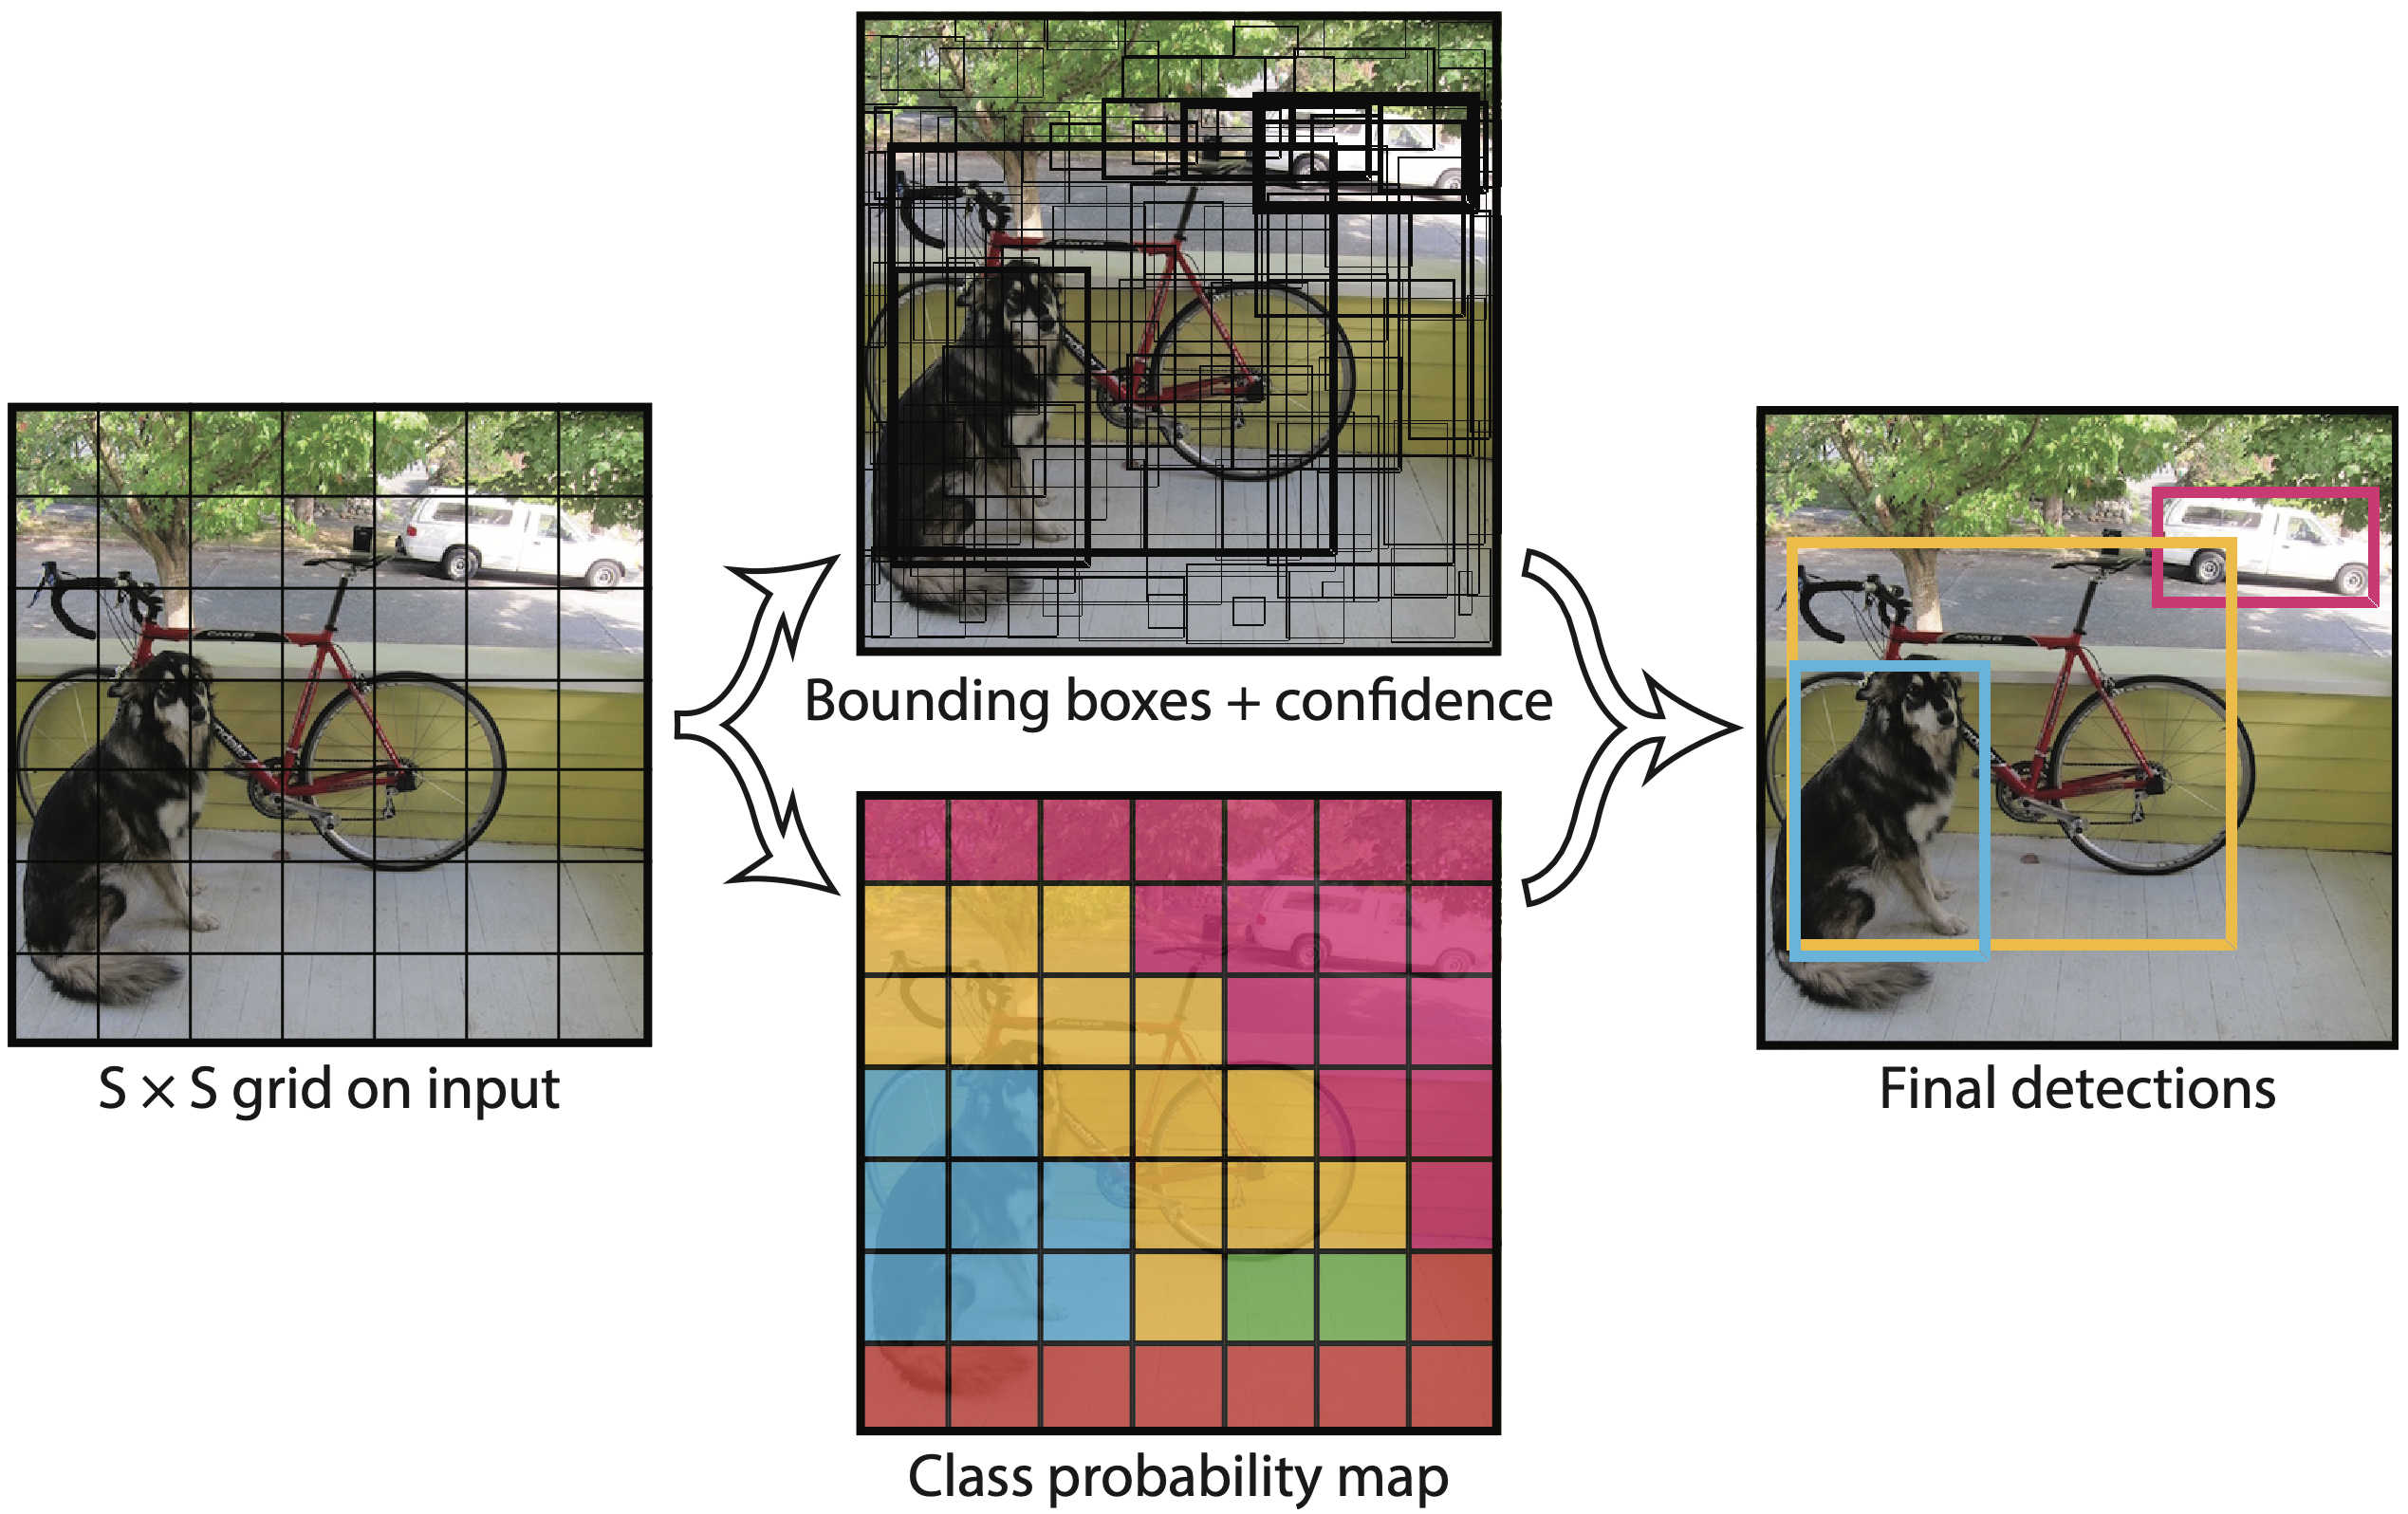
\includegraphics[width=\columnwidth]{images/yolo-model.png}
    \end{center}
    \caption{Pipeline of YOLO presented in \cite{redmon2016you}.}
    \label{fig:yolo-model}
\end{figure}

In YOLO, the input image is divided into a $S \times S$ grid and the cell in which the center of the object falls is responsible for the detection of that object.
A grid cell can predict more than one bounding box, where each prediction consists of an array composed by 5 elements: center of the bounding identified by the coordinates $x$ and $y$, dimensions of the box $w$ and $h$, and the confidence score of that bounding box representing and object. At the same time, regardless of the number of boxes in each cell, C conditional probabilities $\Pr(Class_i | Object)$ are computed in each grid cell. The final prediction will be encoded as an $S \times S \times (B * 5 + C)$ tensor. The model pipeline is shown in \autoref{fig:yolo-model}


\vspace{1.5\baselineskip}
::: TODO ::: Spiegare la loss di YOLO!


Over the years, several versions of YOLO have came up, starting from the first up to fifth versions \cite{redmon2016you, redmon2017yolo9000, redmon2018yolov3, bochkovskiy2020yolov4, glenn_jocher_2021_5563715}. YOLOv5 represents the state of the art for object detection, and compared with the most recent detectors architectures it is among the best performing models \cite{zaidi2022survey}.

\section{Logo recognition}
\label{sec:sota-logoyolo}

A general pipeline for logo detection and recognition consists in logo region proposal followed by a classifier specifically trained for logo classification, as proposed by Bianco et al. in \cite{bianco2017deep} or by Fehérvári et al. in \cite{fehervari2019scalable}.

Another approach presented by Wang et al. \cite{wang2022logodet} involve a model based on YOLOv3 \cite{redmon2018yolov3} used to produce both bounding boxes and classification for each detected logo. The proposed model is called Logo-YOLO, which is essentially the same version of YOLOv3 with some changes to the loss function and the re-computation of the anchors sizes. The modified loss function utilizes the Focal Loss \cite{lin2017focal} to solve the problem of logos usually begin small object relative to the background, and the  CIoU loss \cite{zheng2020distance} to obtain more accurate regression results.

The issue with this approaches is the closed-world assumption which does not apply in the case of logo recognition, as discussed in \autoref{sec:logodet-intro}. This is the motivation behind works such as \cite{fehervari2019scalable}. The authors of the paper propose a method based on Distance Metric learning (DML) using deep learning techniques called SoftTriple Loss and presented in \cite{qian2019softtriple}. This work aims to achieve logo recognition via metric learning, where a model learns the similarity among arbitrary groups of data, thus being able to deal with a large number of previously unseen classes.

Another work based on DML has been presented by Li et al. \cite{li2022seetek} and can be considered as an extension to \cite{fehervari2019scalable}. In this work the author enrich the latent space learned by DML with text features contained in the logos. The authors point out how many logos have remarkable amount of text or (stylized) letters, for this reason they consider both visual and text features for logo classification.

\section{Class incremental learning}
Catastrophic forgetting
\subsection{DER: an algorithm for class incremental learning}
\subsubsection{Algorithm description}
\subsubsection{Weight aligning}
\subsubsection{Masking and pruning}
